%=================
\chapter{Sprint 2}
%=================
This chapter descriptes the results and process of sprint 2. In 
\autoref{sec:sp2:pre} the planed changes from the first sprint is explained, 
the planning of this sprint is covered in \autoref{sec:sp2:planning}, and the 
design of the first sprint is explained in \autoref{sec:sp2:design}. To give a 
better understanding of the requirements, \autoref{sec:sp2:impl} explains the 
features implemented in this sprint. The results from the tests done is 
described in \autoref{sec:sp2:test}. The feedback from the customer is covered 
in \autoref{sec:sp2:feedback}. In \autoref{sec:sp2:eval} the results from the 
sprint retrospective is covered.

%-------------------
\section{Pre-sprint}
%-------------------
\label{sec:sp2:pre}
Sprint 1 gave the desired result, but the team was not satisfied with the way the \Gls{scrum} process was conducted, especially the sprint planning. In sprint 1 retrospect we decided to conform more to, in our mind, proper Scrum. We will apply experience and advice from the first sprint, to get a better process. 

In this planning meeting we will try to have more descriptive work items in the sprint backlog. This will ease the process of design, implementation, testing and documentation of the \gls{utility}, and we do not have to redo any parts that will end up in the report in order to assist the reader. We focus on good user stories to ensure that the elements are of a low enough level.


%------------------------
\section{Sprint Planning}
%------------------------
\label{sec:sp2:planning}
The first sprint resulted in a solid core for the \gls{utility}. During the next sprint iteration, the core will be extended with more advanced functionality. After this sprint, the \gls{utility} will have most of the functionalities it need to work in a real environment, and will probably be able to aid Thales in some of their operations.

Since it is difficult to the understand the complexity of all the requirements in the sprint backlog, the team ended in up with an uncertain person-hours estimate for some work objects. After the sprint is finished, we will see if we understood the complexity, and assigned enough hours to implement it. The more complex, but not so critical functionalities will be part of sprint 3 and 4.   

\subsection{Duration}
%--------------------
According to the work breakdown structure, \autoref{tab:wbs}, the planning meeting of the second sprint should have been conducted the 5th of October. After a request from the customer to see our planning for the second sprint at the weekly customer meeting, which was scheduled to be before our planning meeting the same day, we decided to advance the planning to the 4th of October. This is to maintain the good relationship to the customer and submit to their preference.

The sprint started with the planning meeting the 4th of October and our work started the following day. The sprint duration is 14 days, and will end the 18th of October with a review meeting.  

\subsection{Sprint Goal}
%-----------------------
The second sprint will build on the core created in the first sprint. During the sprint we will extend the functionality with more comprehensive and advanced features. Most of the requirements we intend to fulfill in this sprint had to be done subsequent to the first sprint, because the structure and design of the core had to be in place first. The requirements that we selected for this sprint are a natural advancement on the road to making the \gls{utility} that the customer wants. 

One of the most crucial functions to work in a real environment, is the support for nested \gls{header}-files. The handling of the \gls{include}-statement gives the \gls{utility} this feature. The goal of the sprint is to implement the \gls{include} and mainly to have support for \glspl{enum}, \glspl{bit string}, \gls{endianness} and \gls{batch mode}. 

\subsection{Back Log}
%--------------------
\label{sec:sp2backlog}
The second sprint we will implement thirteen requirements. These are listed in Table
\ref{tab:sprint2req1} and Table \ref{tab:sprint2req2}.

\begin{table}[!htb] \small \center
\caption{Sprint 2 Requirements\label{tab:sprint2req1}}
\begin{tabularx}{\textwidth}{l l X c c}
	\toprule
	& & & \multicolumn{2}{c}{Hours} \\
	\cmidrule(r){4-5}
	\# & Req. & Description & Est. & Act. \\
	\midrule
	1 & FR1-B & Support \glspl{member} of type \glspl{enum} & \underline{ 6 } & 5 \\
	   &  & Implementation & 3 & 2 \\
	   &  & Testing - unit & 1 & 1 \\
	   &  & Testing - end to end & 2 & 2 \\
	\addlinespace
	2 & FR1-C & Support \glspl{member} of type \glspl{struct} & \underline{ 7 } & 3.5 \\
	   &  & Implementation & 6 & 3 \\
	   &  & Testing - unit & 1 & 0.5 \\
	\addlinespace
	3 & FR1-F & Detect \glspl{struct} with same name & \underline{ 3 } & 3.5 \\
	   &  & Implementation & 2 & 2.5 \\
	   &  & Testing - unit & 1 & 1 \\
	\addlinespace
	4 & FR2-B & Support display of \glspl{struct} within \glspl{struct} & \underline{ 11 } & 15 \\
	   &  & Implementation & 5 & 6 \\
	   &  & Testing - unit & 2 & 2 \\
	   &  & Testing - end to end & 4 & 7 \\
	\addlinespace
	5 & FR4-F & Support \glspl{enumerated named value} & \underline{ 5 } & 6.5 \\
	   &  & Design & 1 & 0.5 \\
	   &  & Implementation & 1 & 0.5 \\
	   &  & Testing - unit & 1 & 2.5 \\
	   &  & Testing - end to end & 1 & 1.5 \\
	   &  & User documentation & 1 & 1.5 \\
	\addlinespace
	6 & FR4-G & Support for \glspl{bit string} & \underline{ 10 } & 11.5 \\
	   &  & Design & 2 & 2 \\
	   &  & Implementation & 3 & 6 \\
	   &  & Testing - unit & 2 & 1 \\
	   &  & Testing - end to end & 2 & 1 \\
	   &  & User documentation & 1 & 1.5 \\
	\addlinespace
	7 & FR1-E & Support \glspl{member} of type \gls{array} & \underline{ 7 } & 12 \\
	   &  & Implementation & 3 & 7 \\
	   &  & Testing - unit & 1 & 1 \\
	   &  & Testing - end to end & 3 & 4 \\
	\bottomrule
\end{tabularx}
\end{table}

\begin{table}[!htb] \small \center
\caption{Sprint 2 Requirements continued\label{tab:sprint2req2}}
\begin{tabularx}{\textwidth}{l l X c c}
	\toprule
	& & & \multicolumn{2}{c}{Hours} \\
	\cmidrule(r){4-5}
	\# & Req. & Description & Est. & Act. \\
	\midrule
	8 & FR4-E & \Glspl{struct} with various \gls{trailers} & \underline{ 18 } & 15 \\
	   &  & Design & 3 & 2 \\
	   &  & Implementation & 6 & 6 \\
	   &  & Testing - unit & 2 & 1.5 \\
	   &  & Testing - end to end & 5 & 3.5 \\
	   &  & User documentation & 2 & 2 \\
	\addlinespace
	9 & FR4-B & Support for custom \Gls{lua} configuration & \underline{ 14 } & 7 \\
	   &  & Design & 2 & 1 \\
	   &  & Implementation & 5 & 5 \\
	   &  & Testing - unit & 1 & 0 \\
	   &  & Testing - end to end & 4 & 1 \\
	   &  & User documentation & 2 & 0 \\
	\addlinespace
	10 & FR4-D & \Gls{dissector} ID & \underline{ 4 } & 3 \\
	   &  & Implementation & 1 & 1 \\
	   &  & Testing - unit & 1 & 1 \\
	   &  & User documentation & 2 & 1 \\
	\addlinespace
	11 & FR5-C & \Gls{endian} handling & \underline{ 11 } & 0.5 \\
	   &  & Implementation & 5 & 0.5 \\
	   &  & Testing - unit & 2 & 0 \\
	   &  & Testing - end to end & 6 & 0 \\
	\addlinespace
	12 & FR6-C & Batch processing; folder support in the \gls{cli} & \underline{ 7 } & 4.5 \\
	   &  & Implementation & 4 & 2 \\
	   &  & Testing - unit & 2 & 1.5 \\
	   &  & User documentation & 1 & 1 \\
	\addlinespace
	13 & FR4-C & Support custom handeling of specific data types & \underline{ 5 } & 3 \\
	   &  & Implementation & 2 & 1.5 \\
	   &  & Testing - unit & 1 & 0.5 \\
	   &  & Testing - end to end & 1 & 1 \\
	   &  & User documentation & 1 & 0 \\
	\addlinespace
	14 &  & Non-requirement programming tasks & \underline{ 26 } & 25.5 \\
	   &  & Refactoring & 3 & 7 \\
	   &  & Bug fixing & & 2 \\
	   &  & Manual end-to-end tests & 8 & 4 \\
	   &  & Automatic end-to-end tests & 4 & 3 \\
	   &  & Misc unit tests & 4 & 3 \\
	   &  & Misc user documentation & 7 & 6.5 \\
	\midrule
	& & Total: & 134 & 115.5 \\
	\bottomrule
\end{tabularx}
\end{table}


\begin{table}[!htb] \small \center
\caption{Sprint 2 Timetable\label{tab:sprint2time}}
\begin{tabularx}{\textwidth}{X c c}
	\toprule
	& \multicolumn{2}{c}{Hours} \\
	\cmidrule(r){2-3}
	Description & Est. & Act. \\
	\midrule
	\textbf{Sprint planning} & \textbf{30} & \textbf{35.5} \\
	\addlinespace
	\textbf{Sprint 2 requirements} & \textbf{134} & \textbf{115.5} \\
	Design & 8 & 5.5 \\
	Implementation & 44 & 43 \\
	Testing & 46 & 35 \\
	User Documentation & 10 & 6.5 \\
	Other & 26 & 25.5 \\
	\addlinespace
	\textbf{Sprint review} & \textbf{20} & \textbf{17.5} \\
	\addlinespace
	\textbf{Report documentation} & \textbf{58} & \textbf{69} \\
	Sprint 1 document & 14 & 5 \\
	Sprint 2 document & 44 & 54 \\
	Report document & & 10 \\
	\addlinespace
	\textbf{Lectures} & \textbf{25} & \textbf{27.5} \\
	\addlinespace
	\textbf{Meetings} & \textbf{55} & \textbf{48} \\
	Advisor meetings & 28 & 26 \\
	Customer meetings & 6 & 8 \\
	Stand-up meetings & 21 & 14 \\
	\addlinespace
	\textbf{Project Managment} & \textbf{20} & \textbf{40} \\
	\midrule
	Total: & 342 & 353 \\
	\bottomrule
\end{tabularx}
\end{table}


%----------------------
\section{System Design}
%----------------------
\label{sec:sp2:design}
For sprint 2 the team decided to refactor some of the code in order to make it easier to read and to split the functionalities of the \gls{utility} in such a way that it reduces coupling within the system. Some new functionality was also added on the \gls{parser} side in order to get the \gls{utility} to recognize the datatypes mentioned in the sprint 2 backlog. This new functionality is represented by the addition of new classes in the \gls{dissector} and config modules. These classes include the BitField, ArrayField, EnumField and ProtocolField classes, which contain the functionality required to handle Bitstrings, \glspl{array}, \glspl{enum} and \glspl{struct} within \glspl{struct} respectively. The classes added to the config module include the Trailer, Bitstring, Custom and Enum classes which handles the configuration needs for \glspl{struct} with \gls{trailers}, \glspl{bit string}, custom handling of data types and \glspl{enum} respectively. Other than that, there were no other changes or additions made to the design during sprint 2.

\subsection{Utility}
%--------------------
\autoref{fig:sp2:class} shows the class diagram the team made for sprint 2. 
The main differences from sprint 1 are the additions of new classes, extending 
the functionality of the \gls{utility} so it can handle 
more complex \gls{header} files than it could before. The developers also 
generalized some of the modules and used inheritance to support the re-use of 
code.

The addition to the class diagram have been mainly to support more data types 
for C in the cparser and support for more configuration options in config 
module, and generation of the fields in dissector module.
 
\begin{figure}[!htb]
	\center
	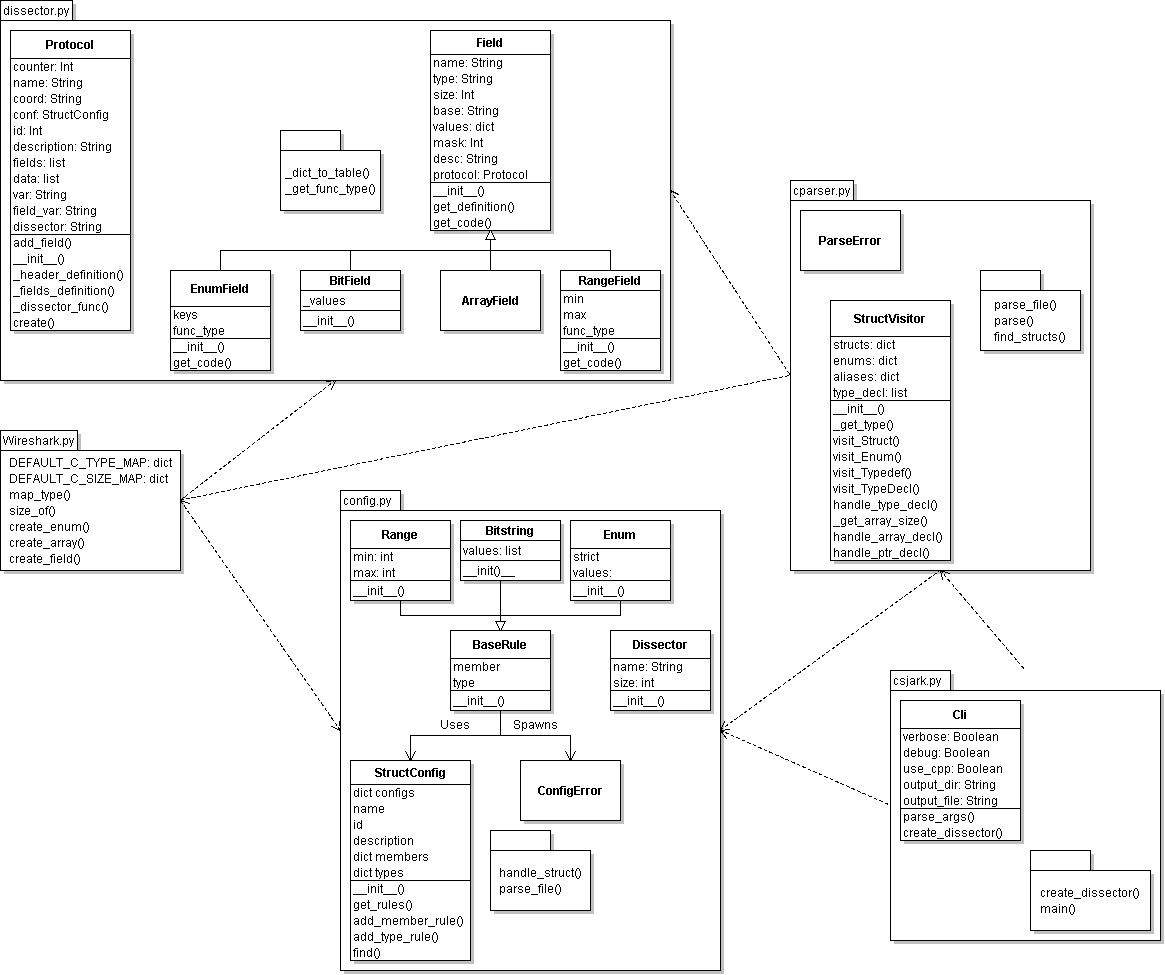
\includegraphics[width=\textwidth]{./sprints/img/class_diagram_s2}
	\caption{Class Diagram\label{fig:sp2:class}}
\end{figure}

\subsubsection{CSjark}
The main differences in this module was changes in the Cli class, which now 
has functionality to find all files in a folder given as an argument when 
running CSjark, with the \emph{files\_in\_folder()}. This method used for the 
support of batch mode generation.

\subsubsection{Cparser}
In the cparser module, there was added a class names ParserError, the main 
thing class to is to raise an exception when our utility do not support a C 
data type. StructVisitor has been extended to support more data types, for 
example structs, arrays and enums.

\subsubsection{Config}
For all the configuration added in this sprint, there has been added a class 
for each configuration. For this there has been added a superclass, named 
BaseRule. This class have all the functionality that the configuration rules 
shares. 

BaseRule has five subclasses, Custom, Enum, Range, Bitstring and Trailer. 
These subclasses have the configuration that are specific for these 
configuration types.

The last class added in this module is ConformanceFile, which hold the 
configuration written for custom Lua code. 

\subsubsection{Dissector}
There was added four subclasses of Field in the dissector module. This classes 
is EnumField, ArrayField, BitField and ProtocolField, these classes will 
generate different types of field for the Lua dissector, that will display 
members differently in Wireshark.

Field and Protocol classes has been extended to support the new fields, and 
support for modifying configuration of the functionality in Wireshark.

\subsection{User stories}
%---------------------------
\label{sec:req:stories2}
This section lists the user stories for the second sprint, these are displayed in \autoref{tab:req:stories3}, \autoref{tab:req:stories4},
\autoref{tab:req:stories5} and \autoref{tab:req:stories6}.
As we are developing a very technical \gls{utility} we have written user stories with an implementation level of abstraction. 
These user stories represent how we intend to add the functionality of each requirement to the \gls{utility}.
The administrator in this context is the administrator at Thales Norway AS. 
The developer is the person that uses \Gls{wireshark} with the \gls{dissector} generated by CSjark.

\begin{table}[htbp] \footnotesize \center
\caption{User stories - Sprint 2 part 1\label{tab:req:stories3}}
\noindent\makebox[\textwidth]{%
\begin{tabularx}{1.2\textwidth}{l X}
	\toprule
	Header & Value \\
	\midrule
	ID & US09 \\
	Requirement & FR1-B: The \gls{utility} must support \glspl{member} of type \gls{enum} \\
	What & The administrator wants the \gls{utility} to support \glspl{struct} with \glspl{member} of type \gls{enum}. \\
	How & When the cparser module detects an \gls{enum} \gls{member} in a \gls{struct}, the cparser should search in an \gls{enum} dictionary and the \gls{enum} \gls{member} 
		will be mapped to the correct value found in the dictionary. A field representing the \gls{enum} will be added to the prototype object corresponding
		to the enclosing \gls{struct}. \\
	Result & The \gls{utility} supports \glspl{member} of type \gls{enum}. \\
	\midrule
	ID & US10 \\
	Requirement & FR1-C: The \gls{utility} must support \glspl{member} of type \gls{struct} \\
	What & The administrator wants the \gls{utility} to support \glspl{struct} with \glspl{member} of type \gls{struct}. \\
	How & When the cparser module detects a \gls{struct} in the AST that has a \gls{struct} \gls{member}, the cparser searches for its definition in the 
		dictionary of previously detected \glspl{struct}. When it finds it, it looks up the identification number and the size of the inner \gls{struct} and creates a 
		struct\_field object with that information inside the prototype object corresponding to the outer \gls{struct}. \\
	Result & The \gls{utility} supports \glspl{member} of type \glspl{struct}. \\
	\midrule
	ID & US11 \\
	Requirement & FR1-F: The \gls{utility} should detect \glspl{struct} with the same name, and report it as an error \\
	What & The administrator wants the \gls{utility} to report an error if it discovers \glspl{struct} with the same name to avoid unforeseen name collisions. \\
	How & When the cparser module traverses the AST to look for \glspl{struct}, it will detect if there are \glspl{struct} with the same name by searching in a database 
		of all \glspl{struct} it has found so far. If a collision is detected the \gls{utility} will crash with an error message. \\
	Result & The \gls{utility} will detect duplicated name of \glspl{struct}. \\
	\midrule
	ID & US12 \\
	Requirement & FR2-B: The \gls{dissector} shall be able to support \glspl{struct} within \glspl{struct} \\
	What & The \gls{utility} should be able to create a \Gls{lua} \gls{dissector} that correctly
	displays \glspl{struct} within \glspl{struct} in \Gls{wireshark}. \\
	How & For each \gls{struct} definition encountered in cparser, a prototype object is created. This object will include an 	identifier number used to locate
		the \Gls{lua} \gls{dissector} for that \gls{struct}. When a \gls{struct} \gls{member} is located inside an outer \gls{struct}. The \gls{dissector} module encodes the identification number 
		and the size for the inner \gls{struct} into the \Gls{lua} \gls{dissector} for the outer \gls{struct}. The identification number is used to access the \gls{dissector} for the inner
		\gls{struct} when the outer \gls{struct} \gls{dissector} is used. The outer \gls{struct} \gls{dissector} uses the size of the inner \gls{struct} to know how much of the network package
		to forward to the inner \gls{struct} \gls{dissector}. The size and identification number of the inner \gls{struct} will be available in the \gls{struct} field corresponding to
		the inner \gls{struct} inside the \gls{protocol} object corresponding to the outer \gls{struct}.  \\
	Result & The \gls{dissector} module supports nested \glspl{struct} \\
	\midrule
	ID & US13 \\
	Requirement & FR4-F: Configuration must support integer \glspl{member} which represent an enumerated named value \\
	What & The administrator wants to specify integer \glspl{member}, represented by an enumerated named value, in a configuration file. \\
	How & The config module should read config files provided to the command line interface, and find any rules regarding enumerated integer values.
		The rules are used by the cparser when it translates 	\gls{struct} definitions to Protocol, and makes the cparser create EnumFields instead of normal
		Fields for the specified \glspl{member}. \\
	Result & Enum \glspl{member} can be specified in the configuration. \\
	\bottomrule
\end{tabularx}}
\end{table}

\begin{table}[htbp] \footnotesize \center
\caption{User stories - Sprint 2 part 2\label{tab:req:stories4}}
\noindent\makebox[\textwidth]{%
\begin{tabularx}{1.2\textwidth}{l X}
	\toprule
	Header & Value \\
	\midrule
	ID & US14 \\
	User doc & FR4-F: User documentation for writing configuration for integer \glspl{member} which represent an enumerated named value. \\
	What & The administrator should be able to educate himself of how to give CSjark the necessary information to get integer values mapped to names in the generated \gls{dissector}. \\
	How & The administrator opens the user documentation and finds the section about configuration. From here he locates the sub section about enumerated names integer values.
	This section gives a good description of how to write such configuration, and the user is able to implement his desired configuration after reading through
	once and looking at provided examples. \\
	Result & The administrator is now able to use the enumerated named value functionality. \\
	\midrule
	ID & US15 \\
	Requirements & FR4-G: Configuration must support \glspl{member} which are \glspl{bit string} \\
	What & The administrator wants to specify \glspl{member} that represent \glspl{bit string} in the configuration. \\
	How & The config module should read config files provided to the command line interface, and find any rules regarding \glspl{bit string}.
	The rules are used by the cparser when it translates \gls{struct} definitions to Protocol and BitField instances found in the \gls{dissector} module. \\
	Result & The administrator can specify \gls{bit string} \glspl{member} in the configuration. \\
	\midrule
	ID & US16 \\
	User doc & FR4-G: User documentation for writing configuration for integer \glspl{member} which are \glspl{bit string}. \\
	What & The administrator should be able to educate himself of how to give CSjark the necessary information to get integer values mapped to \gls{bit string} in 
	the generated \gls{dissector}. \\
	How & The administrator opens the user documentation and finds the section about configuration. From here he locates the sub section about \gls{bit string}
	 integer values. This section gives a good description of how to write such configuration, and the administrator is able to implement his desired configuration
	after reading through once and looking at provided examples.  \\
	Result & The administrator is now able to configure CSjark to generate \gls{dissector} that recognises and formats \glspl{bit string} correctly. \\
	\midrule
	ID & US17 \\
	Requirements & FR1-E: The \gls{utility} must support \glspl{member} of type \gls{array} \\
	What & The administrator wants the \gls{utility} to support \glspl{struct} with \glspl{member} of type \gls{array}. \\
	How & When the cparser module finds an \gls{array} declaration, it recursively traverses the tree until till it encounters the bottom of the declaration 
	to discover the size of the \gls{array}. The \gls{parser} module creates an instance of an \gls{array} field with the size and type of the \gls{array}. From the \gls{array} field
	the \gls{dissector} module generates a \gls{dissector} which has a sub tree for each level of the \gls{array}. \\
	Result & The \gls{utility} support \gls{array} \glspl{member} in \glspl{struct}. \\
	\midrule
	ID & US18 \\
	Requirements & FR4-E: Configuration must support various trailers (other registered \glspl{protocol}) \\
	What & The administrator wants to specify trailers to a \Gls{c} \gls{header} file in the configuration. \\
	How & The config module should read config files provided to the command line interface, and find any rules regarding trailers. A \gls{member} in a \gls{struct}
	will say how many \glspl{packet} of other \glspl{protocol} that follows the \gls{header}. In the config-file it is specified which \gls{member} contains this number, and what
 	type of \gls{protocol} the \gls{packet}(s) belong to. When the \gls{dissector} module generates a \gls{struct} containing a trailer, the correct \gls{dissector} for the trailer \gls{packet}(s) 
	will be called for the rest of the buffer. \\
	Result & The \gls{utility} can handle trailer \glspl{packet} following the \gls{header}, specified in the configuration. \\
	\bottomrule
\end{tabularx}}
\end{table}

\begin{table}[htbp] \footnotesize \center
\caption{User stories - Sprint 2 part 3\label{tab:req:stories5}}
\noindent\makebox[\textwidth]{%
\begin{tabularx}{1.2\textwidth}{l X}
	\toprule
	Header & Value \\
	\midrule
	ID & US19 \\
	User doc & FR4-E: User documentation for how to specify trailers (other registered \glspl{protocol}) \\
	What & The administrator should be able to find out how to specify trailers to a \gls{header} \gls{struct} by reading the user documentation. \\
	How & The administrator opens the user documentation and finds the section about configuration. From here he locates the sub section about trailers. 
	This section gives a good description of how to write such configuration for different types of trailers and provides sufficient examples, so that
	it is  clear to the administrator how to write the configuration he needs after reading the section. \\
	Result & The administrator is now able to utilise the trailer feature of CSjark. \\
	\midrule
	ID & US20 \\
	Requirements & FR4-B: Configuration must support custom \Gls{lua} files for specific \glspl{protocol} \\
	What & The administrator wants to specify custom \Gls{lua} files in the configuration, that are to be used in complex cases where our \gls{utility} is unable to generate
	a \gls{dissector} for the \Gls{c} \gls{header}. \\
	How & The config module should read config files provided to the command line interface, and find any rules regarding the use of custom \Gls{lua} files.
	When such a rule is found, the \gls{dissector} module will use the \Gls{lua} code found in the file(s) in addition to its own generated \Gls{lua} code.
	This is done by reading the custom \Gls{lua} file(s) and writing the content to the relevant parts of the \gls{dissector}. \\
	Result & The administrator can specify the use of custom \Gls{lua} file in the configuration. \\
	\midrule
	ID & US21 \\
	Requirements & FR4-C: Configuration must support custom handling of specific types. \\
	What & The administrator will be able to specify that a certain type should be handled in a specific way specified in a configuration file. This configuration must be
 	a \Gls{wireshark} supported lua field. The configuration could both be a global default value for that type, or specific for a \gls{struct} \gls{member}. \\
	How & The config module should read config files provided to the command line interface, and find any rules regarding the use of custom handling of types.
 	It will modify the field added to the prototype field representing the enclosing \gls{struct} with the behaviour specified in the configuration. \\
	Result & The administrator is able to configure custom behaviour for specific types. \\
	\midrule
	ID & US22 \\
	User doc & FR4-C: User documentation for configuring custom handling of specific types. \\
	What & The administrator should be able to find out how to specify custom handling for a specific type by reading the user documentation.\\
	How & The administrator opens the user documentation and finds the section about configuration. From here he locates the sub section about custom type handling. 
	This section gives a good description of how to write such configuration and what kind of configuration that could be done. There should also be some
 	examples to clarify the description. After reading the section, the administrator has a good idea of how to do the desired custom handling. \\
	Result & The administrator is able to use custom handling of specific types. \\
	\midrule
	ID & US23 \\
	Requirements &  FR4-D: Configuration must support specifying the ID of \glspl{dissector} \\
	What & The administrator wants to specify the ID of a \gls{dissector} in a configuration file. \\
	How & When the cparser finds a \gls{struct} in the \gls{AST} it looks for a configuration file for the \gls{struct}. If a config-file is found, the ID of the \gls{dissector}
	is mapped to the ID given in the config-file when generating the \gls{dissector}. \\	
	Result & The administrator can specfiy the ID of \glspl{dissector} in the configuration. \\
	\midrule
	
\end{tabularx}}
\end{table}

\begin{table}[htbp] \footnotesize \center
\caption{User stories - Sprint 2 part 4\label{tab:req:stories6}}
\noindent\makebox[\textwidth]{%
\begin{tabularx}{1.2\textwidth}{l X}
	\toprule
	Header & Value \\
	\midrule
	ID & US24 \\
	Requirements & FR5-C: Generate \glspl{dissector} which support both little and big \gls{endian} platforms \\
	What & The administrator wants the \gls{utility} to produce \glspl{dissector} that can be used on both little and big \gls{endian} platforms. \\
	How & The administrator will specify the platform he is using in a configuration file by adding a message flag and \gls{endian} pair. When the \gls{dissector} for a \gls{struct} is beeng generated,
 	the \gls{dissector} module in CSjark will encode a flag to \gls{endian} dictionary inside the \Gls{lua} \gls{dissector} file. This dictionary will be used to look up the \gls{endian} for a message given 
	its flag. If no \gls{endian} is found in the dictionary, it will use a default value. \\
	Result & The \glspl{dissector} are now able to support messages from platforms with different \gls{endian}. \\
	\midrule
	ID & US25 \\
	Requirements & FR6-C: Command line shall support batch processing of \Gls{c} \gls{header} and configuration files \\
	What & The administrator wants to set up the program to run automatically, so that the program creates \glspl{dissector} from the \Gls{c} \gls{header} and configuration file(s) that are specified. \\
	How & When the administrator feeds the command line with an input argument, \gls{header} or configuration, the \gls{utility} shall check if the input is a single file or a directory (folder). 
	If it is a file, parse it. If it is a folder, retrieve all files in that folder and add them to a list, this list will be sent to the \gls{parser} and all the files will be parsed one after another.
	A directory within a directory should be detected, and traversed recursively. With this approach we can start in a root folder and include all files,
 	independent of the depth. The \gls{batch mode} shall only include files with the extension .h (a \gls{header} file) or .yml (config file), which are the files that are going to be
	parsed as input.   \\
	Result & The administrator can feed the \gls{utility} with folders to make \glspl{dissector} of all the \glspl{header} found, also called \gls{batch mode}. \\
	\bottomrule
\end{tabularx}}
\end{table}


%----------------------
\section{Implementation}
%----------------------
\label{sec:sp2:impl}
In the previous sprint we focused on creating a naive implementation of the 
\gls{utility}. In this sprint the focus was on implementing data types for the 
\Gls{c} programming language and making it possible to configure more options for how 
the \gls{dissector} should function. This section will cover the requirements 
implemented, what the \gls{header} and config files looks like, and what the ''output'' looks like.

To get a better understanding of how the different requirements were implemented,
look at the user stories for sprint 2 in \autoref{sec:req:stories2}.

\subsection{Support Members of Type \gls{enum}}

%----------------------
\label{sec:supportenum}
\Gls{enum} is a type declaration in \Gls{c}, which specifies enumeration constants.  \Gls{enum} 
is supported because it is a basic datatype in the \Gls{c} language. 
\autoref{code:cenum} shows an example of an \gls{enum} in a \Gls{c}-\gls{header} file. The 
\Gls{wireshark} \gls{dissector} will display the named value, making it 
easier to read, an example is shown in \autoref{fig:wscenum}. The red 
rectangle shows the \gls{enumerated named value}.

\begin{figure}[ht]
	\center
	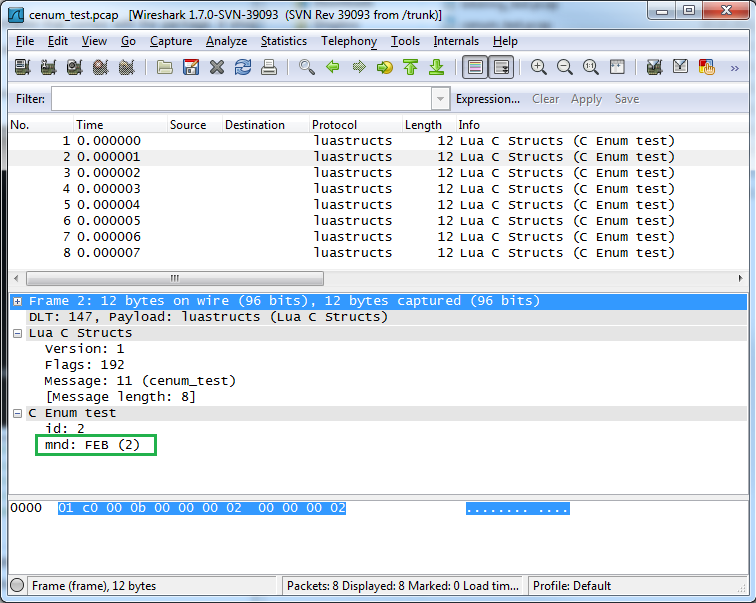
\includegraphics[width=\textwidth]{./sprints/img/wireshark_cenum}
	\caption{Enumeration in \Gls{wireshark}\label{fig:wscenum}}
\end{figure}

\lstset{language=C,caption={\Gls{enum} support},label=code:cenum}
\lstinputlisting[language=C]{./sprints/code/cenum_test.h}

\subsection{Support Members of Type \Gls{struct}}
%----------------------
\Glspl{struct} are an important part of the \Gls{c} language, a \gls{struct} declaration consists 
of a group of different fields, these fields can have any type, also \gls{struct}. 
This was therefore an important requirement to implement. An example is shown 
in \autoref{code:structmember}.

\lstset{language=C,caption={\Gls{struct} support},label=code:structmember}
\lstinputlisting[language=C]{./sprints/code/struct_member.h}

\subsection{Detect \Glspl{struct} with Same Name}
%----------------------
Two \glspl{struct} can have the same name, and therefore we needed a way of detecting it. 
If the \gls{parser} finds two \glspl{struct} with the same name, an exception is 
raised, and the generation of the \gls{dissector} is terminated.

\subsection{Support display of \glspl{struct} within \glspl{struct}}
%----------------------
The \gls{utility} is able to display \glspl{struct} within a \gls{struct} in \Gls{wireshark}, the 
\gls{member} will be visible, and the \gls{struct} will be in a subtree that can be 
expanded. \autoref{fig:wsstructstruct} is a screenshot of this \gls{dissector} in 
\Gls{wireshark}.

\begin{figure}[ht]
	\center
	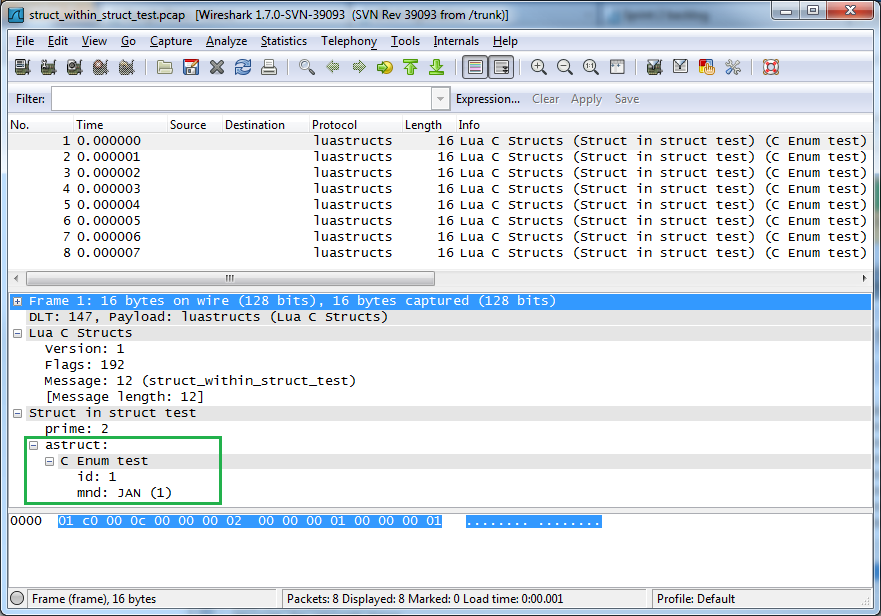
\includegraphics[width=\textwidth]{./sprints/img/wireshark_structwithstruct}
	\caption{\Glspl{struct} in \Gls{wireshark}\label{fig:wsstructstruct}}
\end{figure}

\subsection{Support Enumerated Named Values}
%----------------------
In \Gls{c} there are two ways to do enumerations, the first option was explained in 
\autoref{sec:supportenum}, the other way is to use \gls{define} which is shown in 
\autoref{code:defenum}. The advantage of using \gls{define} is that the values 
can be generated. Since this cannot be understood by the \gls{parser}, it can be 
generated directly from the \gls{header} file, so it have to be supported by 
configuration. \autoref{code:enumconf}. The \gls{enum} will be displayed in 
the same way as in \autoref{sec:supportenum}.

\lstset{language=C,caption={Enumerated named values},label=code:defenum}
\lstinputlisting[language=C]{./sprints/code/def_enum.h}

\lstset{language=C,caption={Enumerated named values config},label=code:enumconf}
\lstinputlisting[language=C]{./sprints/code/def_enum.yml}

\subsection{Support for Bit Strings}
%----------------------
All bits in a basic data type can represent different values. An \gls{integer} is 
represented by 4 bytes(32 bits), each of these bits can for example represent 
32 ''true/false' values. Our \gls{utility} support configuration of these bits. Bits 
can be in groups, so they can represent more than two values. 
\autoref{code:bitstring} shows how \gls{bit string} can be configured. 
\autoref{fig:wsbitstring} shows an example of how \glspl{bit string} are displayed in 
\Gls{wireshark}. Each group of bits is masked, so it is easier to see the values. 
The values are also named, if they are configured.

\begin{figure}[ht]
	\center
	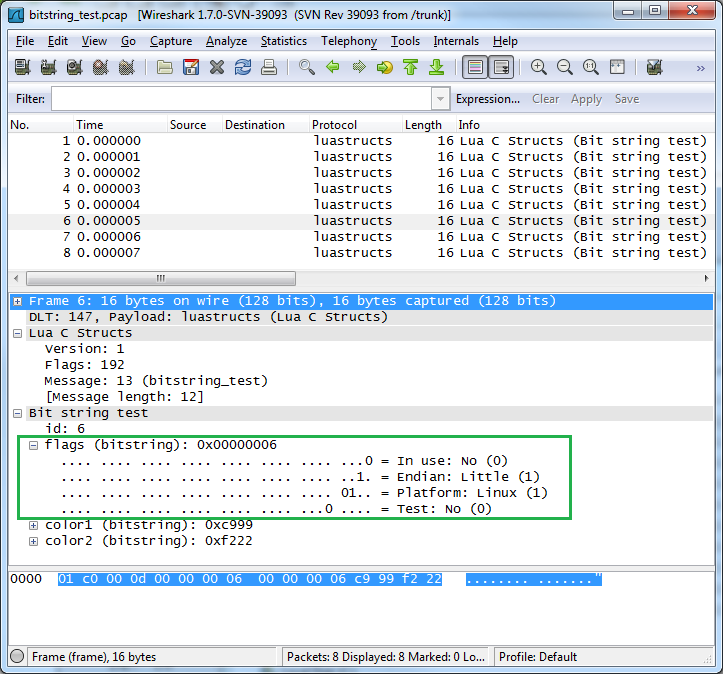
\includegraphics[width=\textwidth]{./sprints/img/wireshark_bitstring}
	\caption{Bit string in \Gls{wireshark}\label{fig:wsbitstring}}
\end{figure}

\lstset{language=C,caption={Bitstring configuration},label=code:bitstring}
\lstinputlisting[language=C]{./sprints/code/bitstring.yml}

\subsection{Support Members of Type \Gls{array}}
%----------------------
Csjark supports \gls{header}-files with \glspl{array}, and is able to display them in 
\Gls{wireshark} with the \Gls{lua}-\gls{dissector}. Csjark supports \glspl{array} of all data types 
implemented so far. The \Gls{wireshark} \gls{dissector} can display multidimensional 
\glspl{array}, and will create a new subtree for each dimension.  A representation of 
\glspl{array} in \Gls{wireshark} is displayed in \autoref{fig:wsarray}.

\begin{figure}[ht]
	\center
	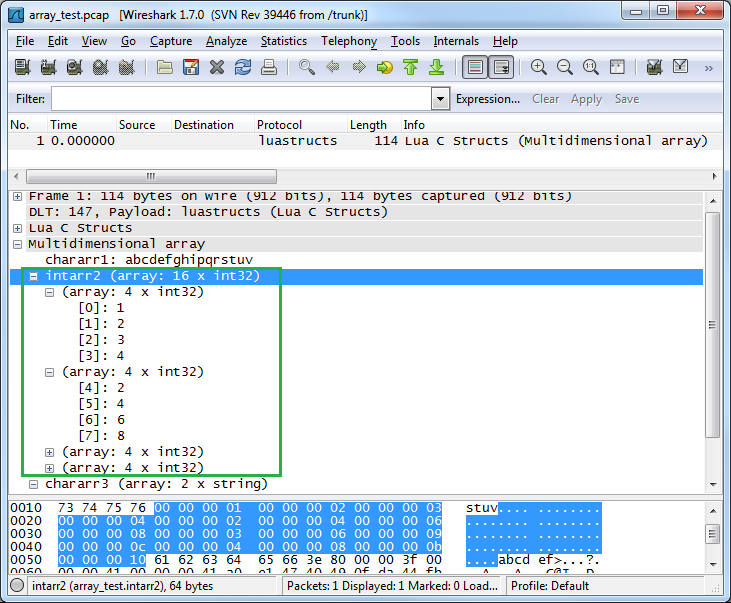
\includegraphics[width=\textwidth]{./sprints/img/wireshark_array}
	\caption{\Glspl{array} in \Gls{wireshark}\label{fig:wsarray}}
\end{figure}

\subsection{\Gls{struct} with Various Trailers}
%----------------------
The \gls{utility} is able to support all kinds of \gls{trailers} that \Gls{wireshark} have 
built-in \glspl{dissector} for. Trailers are data that follows a \gls{struct}, this can be 
any kind of data, but only trails that have built-in support in \Gls{wireshark} can 
be displayed.  To be able to use the \Gls{wireshark} \glspl{dissector}, they have to be 
configured. In the example below, the \Gls{wireshark} \gls{dissector} for \gls{asnone} 
\gls{ber} is used.  In \autoref{code:trailer}, we 
specify ''asn1\_count'' as a \gls{member} in the \gls{struct}, this is used to tell the 
number of \gls{asnone} fields. The config in  \autoref{code:trailerconf} specifies 
fields with size of six bytest, the number of fields are specified by the data 
sent with the \gls{struct}. At the end there is aa field of size five bytes. An 
example of \gls{asnone} in \Gls{wireshark}, can be seen in \autoref{fig:wstrailer}.

\begin{figure}[ht]
	\center
	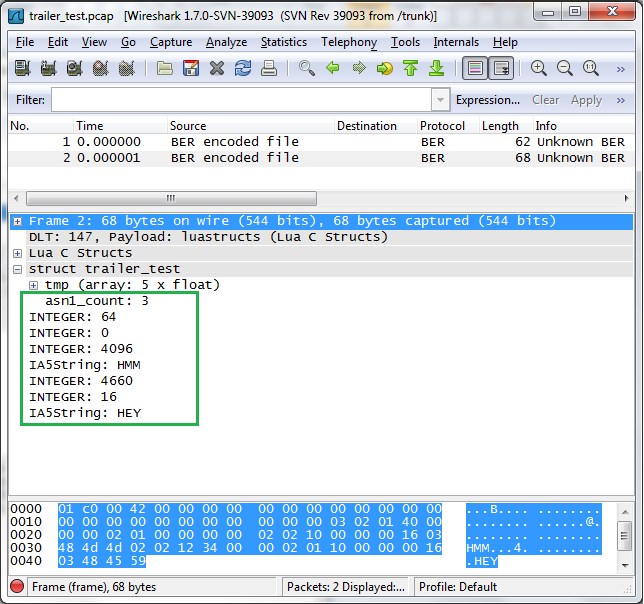
\includegraphics[width=\textwidth]{./sprints/img/wireshark_trailer}
	\caption{\gls{ber} Trailer in \Gls{wireshark}\label{fig:wstrailer}}
\end{figure}

\lstset{language=C,caption={Enumerated named values},label=code:trailer}
\lstinputlisting[language=C]{./sprints/code/trailer.h}

\lstset{language=C,caption={Enumerated named values config},label=code:trailerconf}
\lstinputlisting[language=C]{./sprints/code/trailer.yml}

\subsection{Custom \Gls{lua} Configuration}
%----------------------
Csjark can support custom \Gls{lua} configuration, by including \Gls{lua}-\glspl{script} from a 
file specified in the configuration file. The reason for supporting custom \Gls{lua} 
configuration is for protocols that are not built-in \glspl{dissector} in \Gls{wireshark}, 
and are not \glspl{struct}, or display the members in a struct in a different way 
than our utility do . The only way to support this, is to write \Gls{lua} code for 
it. To be able to insert the \Gls{lua} code in correct places in the lua files, the 
utility use a conformance file, which make it possible to specify where in the 
dissector the code should be inserted. This feature was not completly finished 
in this sprint, and will be finished in sprint 3.

\subsection{\Gls{dissector} ID}
%----------------------
All luastructs-\glspl{packet} that \Gls{wireshark} captures, has a \gls{header}, one of the fields in 
the \gls{header} is the message id. This id is used to load the the correct 
\gls{dissector} when a \gls{packet} is captured. Each \gls{dissector} should have a unique id, 
to avoid possible conflicts. This functionallity is implemented and the 
message id must be specified in the configuration file, \autoref{code:msgid} 
is an example of how this is done.

\lstset{language=C,caption={\Gls{dissector} ID config},label=code:msgid}
\lstinputlisting[language=C]{./sprints/code/messageid.yml}

\subsection{\Gls{endian} Handling}
%----------------------
\Gls{endian} handling is postponed to the next sprint, because it is a platform 
specific problem, and should be implemented together with platform support.

\subsection{Folder Support in the \gls{cli}}
%----------------------
Folder support in the \gls{cli}\footnote{Command-line Interface} has been 
implemented, so it is possible to generate \Gls{lua}-\glspl{script} for all \glspl{struct} stored 
in a given folder. At the moment, all \glspl{dissector} will be regenerated. 
Functionality to only generate modified or new \gls{header}-files will be added in 
the next sprint. \autoref{fig:csjarkfolder} is an example usage of CSjark where
the command first shows the usage of CSjark, and the second command 
generates \glspl{dissector} from the folder ''\gls{header}/'' and configurations from ''etc/''.

\begin{figure}[ht]
	\center
	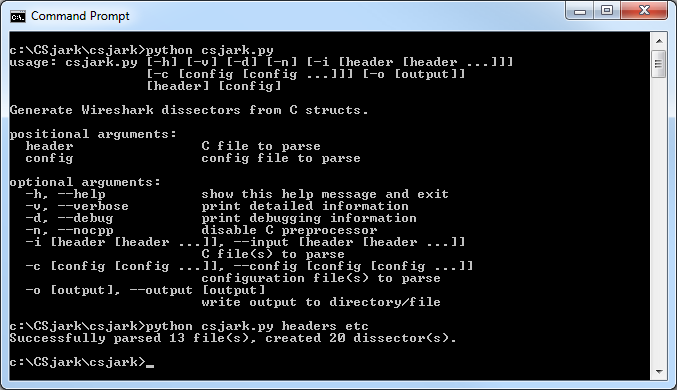
\includegraphics[width=\textwidth]{./sprints/img/csjark_folder}
	\caption{Usage of \Gls{wireshark}\label{fig:csjarkfolder}}
\end{figure}

\subsection{Support Custom Handling of Specified Data Types}
%----------------------
The \gls{utility} supports custom handling of specific data types, this includes 
functionality to support  time\_t and nstime\_t. All basic data types and 
\gls{struct} \glspl{member} can be configured to be handled in a special way. 
\autoref{code:customstruct} show an example of a \gls{struct} with four \glspl{member}, two 
of them are time fields, and the last two is a BOOL and an \gls{integer} to be 
handled in a custom way. This \gls{struct} is configured in 
\autoref{code:customconfig}, in the config the two time fields are configured 
to be respectively absolute time and relative time, and the BOOL type to have 
a size of four bytes. The \gls{struct} \gls{member} ''all' is configured with an enumerated 
value, and will be visible as a hex-value. \autoref{fig:customdatatype} is a 
screenshot of the \gls{struct} in \Gls{wireshark}.

\begin{figure}[ht]
	\center
	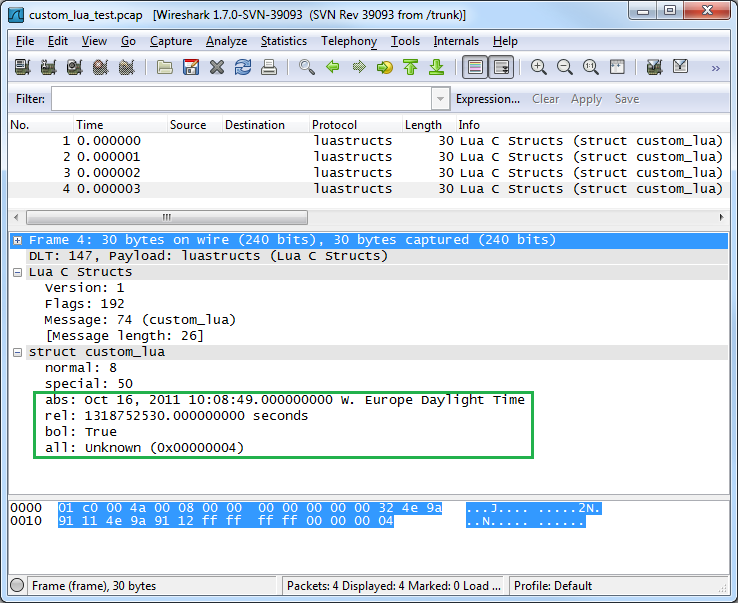
\includegraphics[width=\textwidth]{./sprints/img/wireshark_custom}
	\caption{Custom handling of Data Types\label{fig:customdatatype}}
\end{figure}

\lstset{language=C,caption={\Gls{struct} for custom handling},label=code:customstruct}
\lstinputlisting[language=C]{./sprints/code/customfield.h}

\lstset{language=C,caption={Config for custom handling},label=code:customconfig}
\lstinputlisting[language=C]{./sprints/code/customfield.yml}

\subsection{Typedef Support}
%----------------------
Csjark is supporting the keyword typedef, which is a facility to create new 
data types names. \autoref{code:typedef} shows examples of typedef's that 
csjark supports.

\lstset{language=C,caption={Typedef example},label=code:typedef}
\lstinputlisting[language=C]{./sprints/code/typedef.h}

%-----------------------
\section{Sprint Testing}
%-----------------------
\label{sec:sp2:test}
This section introduces the tests preformed during the sprint and their results. For sprint 2 it was also decided that the larger unit tests should also be documented and added to the test documents.

%subsection{Tests}
During the sprint the team executed a total of 7 test cases with names as seen below. The test cases can be found in \autoref{sec:testcases}. Test cases executed:
\begin{itemize}
	\item TID08 - Supporting \glspl{member} of type \gls{enum} \autoref{tab:sp2TID08}
	\item TID09 - Supporting \glspl{member} of type \gls{array}  \autoref{tab:sp2TID09}
	\item TID10 - Supporting the display of \glspl{struct} within \glspl{struct}  \autoref{tab:sp2TID10}
	\item TID11 - Supporting \glspl{enumerated named value}  \autoref{tab:sp2TID11}
	\item TID12 - Supporting \glspl{bit string}  \autoref{tab:sp2TID12}
	\item TID13 - Supporting \glspl{struct} with various \gls{trailers} \autoref{tab:sp2TID13}
	\item TID14 - Sprint 2 functionality test \autoref{tab:sp2TID14}
\end{itemize}

\subsection{Test Results}
%----------------------------
\begin{table}[!htb] \footnotesize \center
\caption{Recognizing Supporting \glspl{enum} \label{tab:sp2TID08}}
\begin{tabular}{l l}
	\toprule
	Header & Description \\
	\midrule
	Description &  Supporting \glspl{member} of type \gls{enum}  \\
	Tester & Lars Solvoll Tønder \\
	Date & 15.10.2011 \\
	Result & Success\\
	\bottomrule
\end{tabular}
\end{table}

\begin{table}[!htb] \footnotesize \center
\caption{Recognizing Supporting \glspl{array} \label{tab:sp2TID09}}
\begin{tabular}{l l}
	\toprule
	Header & Description \\
	\midrule
	Description &  Supporting \glspl{member} of type \gls{array}   \\
	Tester & Lars Solvoll Tønder \\
	Date & 15.10.2011 \\
	Result & Success\\
	\bottomrule
\end{tabular}
\end{table}

\begin{table}[!htb] \footnotesize \center
\caption{Supporting the display of sctructs within \glspl{struct} \label{tab:sp2TID10}}
\begin{tabular}{l l}
	\toprule
	Header & Description \\
	\midrule
	Description &  Supporting the display of sctructs within \glspl{struct} \\
	Tester & Erik Bergersen \\
	Date & 17.10.2011 \\
	Result & Success. \\
	\bottomrule
\end{tabular}
\end{table}

\begin{table}[!htb] \footnotesize \center
\caption{Supporting enumerated name values \label{tab:sp2TID11}}
\begin{tabular}{l l}
	\toprule
	Header & Description \\
	\midrule
	Description &  Supporting enumerated name values \\
	Tester & Lars Solvoll Tønder \\
	Date & 17.10.2011 \\
	Result & Success\\
	\bottomrule
\end{tabular}
\end{table}


\begin{table}[!htb] \footnotesize \center
\caption{ Supporting \glspl{bit string} \label{tab:sp2TID12}}
\begin{tabular}{l l}
	\toprule
	Header & Description \\
	\midrule
	Description & Supporting \glspl{bit string} \\
	Tester & Lars Solvoll Tønder \\
	Date & 17.10.2011 \\
	Result & Success\\
	\bottomrule
\end{tabular}
\end{table}

\begin{table}[!htb] \footnotesize \center
\caption{Supporting \glspl{struct} with various \gls{trailers} \label{tab:sp2TID13}}
\begin{tabular}{l l}
	\toprule
	Header & Description \\
	\midrule
	Description & Supporting \glspl{struct} with various \gls{trailers} \\
	Tester & Erik Bergersen \\
	Date & 18.10.2011 \\
	Result & Success\\
	\bottomrule
\end{tabular}
\end{table}

\begin{table}[!htb] \footnotesize \center
\caption{Sprint 2 functionality test\label{tab:sp2TID14}}
\begin{tabular}{l l}
	\toprule
	Header & Description \\
	\midrule
	Description & unit test covering all of the functionality implemented in sprint 2 \\
	Tester & Lars Solvoll Tønder \\
	Date & 18.10.2011 \\
	Result & Success\\
	\bottomrule
\end{tabular}
\end{table}

\subsection{Test Evaluation}
%-------------------------------
For the second sprint the developers focused a lot more on testing during implementation. The team also decided that the testers should check how much of the code was covered in the unit tests. This made the group focus more on making proper unit tests that tests as much functionality as possible. This had a very positive effect on the tests that were run at the end of the sprint, where not a single test failed, except for one which ended up exposing a bug in \Gls{wireshark}

\subsection{Test Coverage}
This section introduces the amount of code covered by our unit tests and how it relates to the test coverage from the previous sprints.

\subsubsection{Sprint 1}
As the team had not started measuring code coverage in sprint 1, the testing team had to revert the project to an earlier version and retroactively check the code coverage from the first sprint. The following list contains the unit tests used in the sprint, and the coverage is shown in \autoref{tab:sp1CoverageReport}

\begin {itemize}
\item requirements.py
\item test\_cparser.py
\item test\_csjark.py
\item test\_config.py
\end{itemize}

\begin{table}[!htb]\footnotesize\center
	\caption{Sprint 1 Coverage Report\label{tab:sp1CoverageReport}}
	\begin{tabular}{l l l l l}
		\toprule
		Module & Statements & Missing & Excluded & Coverage\\
		\midrule
		config & 298 & 125 & 0 & 87\%\ \\
		cparser & 215 & 50 & 0 & 74\%\ \\
		csjark & 113 & 57 & 0 & 59\%\ \\
		\gls{dissector} & 460 & 79 & 0 & 38\%\ \\
		Total & 1086 & 311 & 0 & 64\%\ \\
		\bottomrule
	\end{tabular}
\end{table}

\subsubsection{Sprint 2}
The following list contains the unit tests used in the second sprint and the code coverage can be seen in \autoref{tab:sp2CoverageReport}. We also ran a comparizon from the previous sprint and created a chart that we would use to monitor the progress of the code coverage. As can be seen in \autoref{fig:sp2CoverageChart} there was not a tremendous ammount of progress from the previous sprint when it came to code coverage. This is mostly due to the amount of new features that were added this sprint and the fact that using code coverage got implemented very late in the sprint, giving the developers and testers little time to use the metrics to improve the tests.

\begin{itemize}
\item black\_box.py
\item requirements.py
\item test\_config.py
\item test\_csjark.py
\item test\_\gls{dissector}.py
\item test\_cparser.py
\end {itemize}

\begin{table}[!htb]\footnotesize\center
	\caption{Sprint 2 Coverage Report\label{tab:sp2CoverageReport}}
	\begin{tabular}{l l l l l}
		\toprule
		Module & Statements & Missing & Excluded & Coverage\\
		\midrule
		config & 298 & 125 & 0 & 58\%\ \\
		cparser & 215 & 50 & 0 & 77\%\ \\
		csjark & 113 & 57 & 0 & 50\%\ \\
		\gls{dissector} & 460 & 79 & 0 & 83\%\ \\
		Total & 1086 & 311 & 0 & 67\%\ \\
		\bottomrule
	\end{tabular}
\end{table}

\begin{figure}[ht]
	\center
	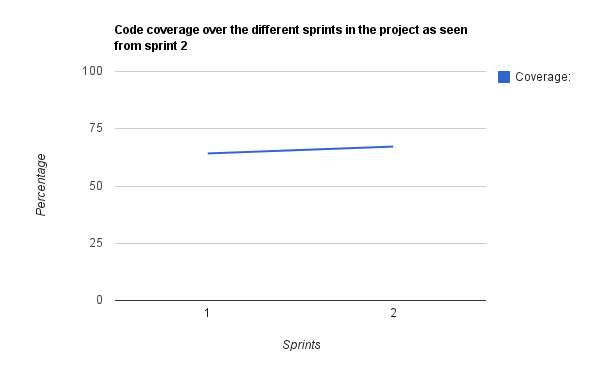
\includegraphics[width=\textwidth]{./sprints/img/sprint2_code_coverage_chart}
	\caption{Code coverage progress from previous sprints\label{fig:sp2CoverageChart}}
\end{figure}


 


%--------------------------
\section{Customer Feedback}
%--------------------------
\label{sec:sp2:feedback}
\subsection{Requirement changes and feedback}
In sprint 2 we were able to demonstrate many of the requirements for the customer, and as a result we got some feedback of some changes and refinements that the customer wants. The customer also added some new features they would like to have. The changes and additions are listed below.

\subsubsection{FR1-E: Support \glspl{member} of type \gls{array}}
\Glspl{array} should be displayed as a sublevel. Multidimensional \glspl{array} should have one sublevel per dimension. The \gls{dissector} should also display the type of the \gls{array} and show the different indexes for the sublevels.

\subsubsection{FR2-B: \gls{struct} within \glspl{struct}}
The customer stated that the inner \gls{struct} should be displayed as a sublevel of the outer \gls{struct}.
When an external \gls{dissector} is called, it should be called with name, and not id, so that \glspl{struct} that is never used as a base does not need to be assigned an id.

\subsubsection{FR4-C Custom handling of specific types}
The customer stated that they would like certain types to be interpreted in a certain way as default behaviour, but that the user should be able to configure specific behaviour for a specific \gls{member} of a \gls{struct}.

\subsubsection{FR4-E: \Glspl{header}/\gls{trailers}}
The customer originally stated that this feature included both \glspl{header} and trailer \glspl{struct} for a given \gls{struct}. This is now refined to mean that the given \gls{struct} is the \gls{header}, and that it can have various \gls{trailers} (could be one or more \Gls{c} \glspl{struct}, \gls{asnone}, etc.). A configuration file should specify the kind of trailer, and what variable inside the \gls{header} \gls{struct} which specify how many trailer items to expect. If the \gls{header} does not specify the length of the trailer the \gls{dissector} should just use the rest of the buffer, or the \gls{dissector} is responsible to return the length used from the buffer, so the caller can give the rest to the next \gls{dissector}.
In \Gls{wireshark} it should be displayed as a sequence of \glspl{struct}.

\subsubsection{FR4-F: Support for \glspl{integer} that represents enumerated values and \glspl{bit string}}
The customer clarified this by explaining that they wanted \glspl{integer} that represents an enumerated value to be displayed like an \gls{enum} (\gls{member} name and the \gls{string} that represents the \gls{integer} value) and that the \glspl{bit string} should be displayed as a list with the name and value (1 / 0 or yes / no) of the different bits in the \gls{integer}. It should also display the original \gls{integer} I hex. As a result of this, the requirement was split into two:
\begin{itemize}
\item FR4-F	Support \glspl{enumerated named value}
\item FR4-G	Support for \glspl{bit string}
\end{itemize}
The customer also confirmed that the \glspl{bit string} are \gls{endian} specific and that they would like them to start counting from 1 (not zero, as in our first implementation).

\subsubsection{FR5-C \Gls{endian} handling}
The customer stated that the \gls{header} part of the \gls{packet}, which include the platform flag, will always be in big \gls{endian} (network order).

\subsubsection{FR7-C: \Gls{batch mode}}
The customer clarified this to mean that the \gls{utility} should be able to run completely unattended given a set of command line arguments. For example it should not ask the users any questions under this mode. This is to be able to run it as a \gls{cron} job at night.

\subsubsection{NR4: A user without prior knowledge should be able to use the tool within X hours.}
The customer defined X as 5.

\subsubsection{NR5: A user with prior knowledge should be able to use the tool within Y hours.}
The customer defined Y as 1.

\subsubsection{Detecting ambiguous \gls{struct} definitions (more than one \gls{struct} definition with the same name)}
The \gls{utility} should detect if there are more that one \gls{struct} with the same name. If found, the \gls{utility} should exit with a proper error message because 

\subsubsection{Data alignment}
The customer said that we could have some problems with alignment with the current offsets, because the different platforms may pad the data \glspl{member} of a \gls{struct} to match an \gls{integer} number of words on that platform.

\subsubsection{Testability}
The customer suggested that we might want to refine some of the requirement to make them more testable. This can be done by adding more measurable goals.

\subsubsection{Documentation}
The documentation should specify what parameters are needed, like what parameters that should be passed to a \gls{dissector}.

\subsubsection{Locating “missing” \gls{header} files}
Some of the \gls{header} files specified in a file might be located in an unknown location. The customer suggested that we should include a way to configure \gls{header} location.

\subsubsection{What \glspl{header} should the \gls{utility} generate \glspl{dissector} for}
The customer suggested that we include a way to specify the relevant \gls{header} files in a configuration file.

\subsubsection{\Gls{dissector} id}
Only \glspl{struct} explicitly configured with an id should be assigned an id. The rest should be called by their textual name. This is to avoid id collisions and limit the amount of configuration needed.

\subsubsection{\Glspl{header} and configuration the \gls{utility} cannot handle}
The customer stated that they wanted the tool to continue generating \glspl{dissector} even if it encounters a file it cannot handle. The tool should just give an appropriate error message and carry on with the next file.

\subsection{Customers feedback on the product}
The customer is satisfied with the progress of the \gls{utility} and is so far pleased with its functionality. They also feel that the team are flexible when it comes to feature refinement and additions. 

%--------------------------
\section{Sprint Evaluation}
%--------------------------
\label{sec:sp2:eval}
This section contains the team evaluation of the second sprint.

\subsection{Review}
%--------------------------
The first sprint evaluation resulted in some planned actions for the forthcoming sprints. Looking back at these at now, we quickly realized that we fell into the same pitfalls again: lack of documentation, bad work distribution and reverse engineering of vital parts.

The sprint started out very good. We had a four-hour long planning meeting, and ended up with a good backlog and a common understanding of the technical aspects of the sprint. Even though the meeting was significantly better this time, we failed in doing the design early. User stories was postponed till the middle of the sprint and they were written by team members that had no understanding of the code. Doing them in a reverse engineered fashion ended up being more work than expected. This is something that we definitely have to change in the next sprints, if we want to do Scrum properly.

The rest of the sprint went as expected. Implementation went smoothly and the customer is satisfied with our progress.

The planned improvement in the documentation part was not followed up. We did more documentation than in the first sprint, but we had problems gathering it together so that the advisers could look at it. In this way we lost a lot of valuable feedback. We have to focus on this the next sprint.

In our sprint backlog, that we made at the sprint planning meeting, we listed responsible for each task. In retrospect this did not work out very well. The problem we encountered was that the most experienced programmer took almost all the programming tasks, leaving documentation tasks for the rest of the team. This could have worked out well, if the documentation and implementation were independent of each other. We know that the implementation and documentation are highly dependent, and that it is not easy to write documentation for code you have not written yourself. So all team members had to ask the implementer how he did it and how it works, which was not very efficient. 
This actually resulted in two bad experiences:
\begin{itemize}
\item Work distribution was uneven. Those with responsibilities were expected to do their task, but we did not think that a task might have been poorly estimated. Some tasks which seemed simple ended up being hard and consumed a lot of person hours.
\item Not all items in the sprint backlog were completed. Because of the uneven work distribution, we realised too late that some of the backlog items would take considerable more time to complete. The person responsible for a task might have had a lot of other tasks that he needed to complete before starting on the current task, and thereby he could not get help from the other team members to complete it.
\end{itemize} 
 All in all we feel that we are still learning to do Scrum properly and if we take the new planned actions in true consideration, we most likely will perform considerable better at the next iteration. 
\\
\\
The burndown chart, \autoref{fig:sp2:burndown}, shows the progress during the second sprint. The estimation seem bad, but since we postponed one of the work items it does not reflect the true actual hours left. The postponed item was estimated 13 hours. Then the sprint end up being 27-13=14 actual hours left. We feel that the estimations, if we exclude the postponed work item, were good and accurate.
\begin{figure}[!htb]
	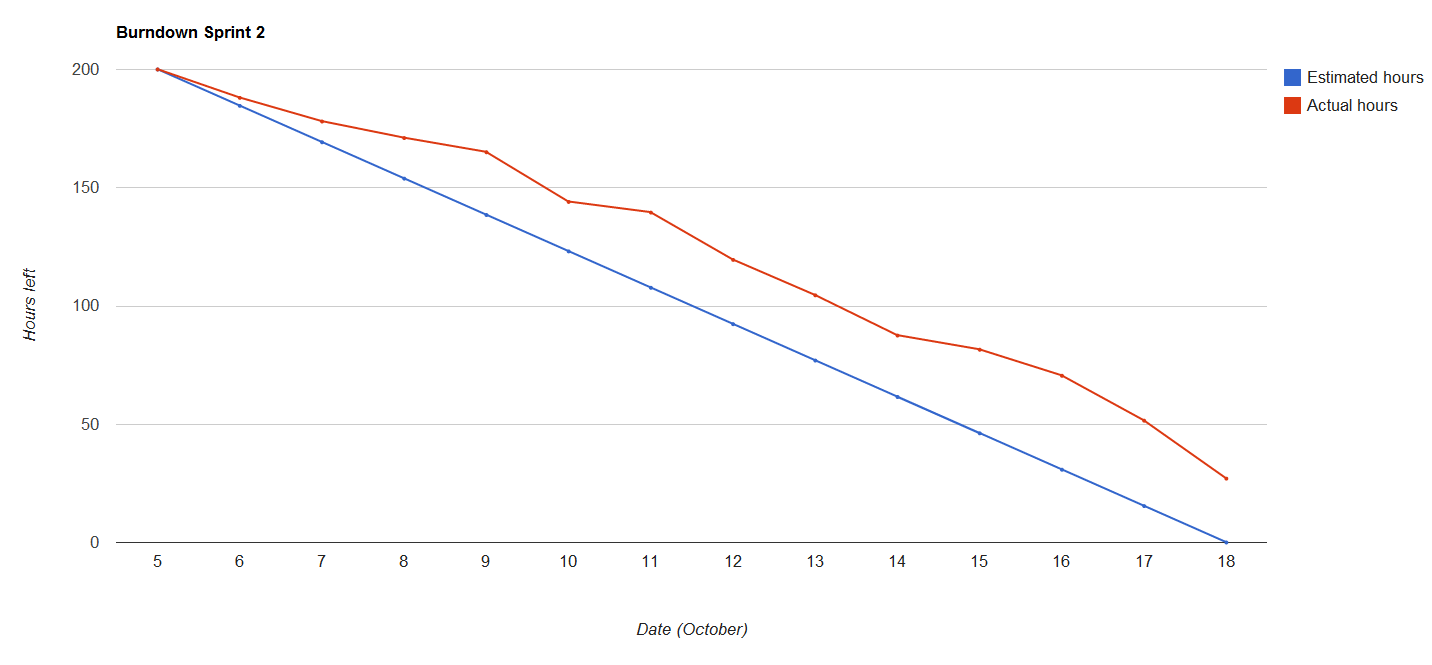
\includegraphics[width=\textwidth]{./sprints/img/burndown_chart_s2}
	\caption{Burndown chart\label{fig:sp2:burndown}}
\end{figure}



\subsection{Positive Experiences}
%--------------------------
\begin{itemize}
	\item A significantly better sprint planning meeting
	\item All the team members have raised their effort, working more hours
	\item Accurate time estimates for most of the work items
	\item Successful presentation of the \gls{utility} to the customer
	\begin {itemize}
		\item Implementation of features are as intended
		\item Good feedback from the customer
	\end{itemize}
	\item Thriving team atmosphere
\end{itemize}



\subsection{Negative Experiences}
%--------------------------
\begin{itemize}
	\item The planning meeting was too short, which resulted in a shortcoming in the documentation.
	\item Documentation was postponed till the end again
	\item Lack of feedback to the advisor
	\item Poor work balance
	\item Could not complete all the tasks in the backlog
\end{itemize}


\subsection{Planned Actions}
%--------------------------
We intend to complete these planned actions for the next sprint. To achieve better performance it is crucial that the importance of these actions are not neglected.

\subsubsection{Do the design in the planning}
Last evaluation meeting we agreed to do the design early in the sprint. Since that did not work for us, we have decided to do the design in the planning meeting. Then it will not be possible to postpone it and the rest of the work will be more efficient. We will use as many hours as it takes to have a planning meeting where we end up with a good plan, proper documentation and detailed user stories.

\subsubsection{Not assign responsibilities}
We will not assign responsibilities for all the tasks at the sprint planning meeting, we rather assign responsibilities for one task for each team member. This way no team members can assign themselves a lot of tasks and might in the end realize that they are not able to complete all the tasks. Now all team members will be able to see what is done and what is not, and assign an unassigned task to themselves. We hope that this will make us capable of completing the whole sprint backlog within the given time.

\subsubsection{List dependencies and prioritize the work items}
As some tasks are dependent on others, it is important to understand this early and plan so that no team member must wait for others to do a task. Now that we do not want to assign responsibilities to all tasks, it is crucial to prioritize each task so that we know what tasks to do first. We do not want to end up with undone work items that have a high priority when the sprint is over. These changes are applied to the sprint backlog.

\subsubsection{Provide more and better documentation to the advisers}
We will strive to give our advisers more documentation to look at. We need their feedback and help in order to finish this project in a suitable manner. 


\subsection{Barriers}
%--------------------------
\subsubsection{The work distribution} 
As mentioned in the review, the team had an uneven work distribution. Some team members were eager to start implementing and took all the implementation tasks, leaving mostly documentation tasks for the rest of the team. The documentation tasks are closely connected to the implementation, so this resulted in problems. Documentation were postponed till the end.The planned actions section describes how we are planning to avoid that this happens again. 

\subsubsection{\Gls{wireshark}} 
We identified several bugs in \Gls{wireshark}, which ended up crashing it when we tried to run our \gls{utility}. Most of them were fixed by Stig, as he works as a core developer for \Gls{wireshark}. Unfixed bugs either will be fixed or dropped because they are not really relevant to us. Time can be lost while we wait for a patch.

\subsubsection{Complexity consideration}
As always, design and estimation of future implementation is hard. At the planning meeting, we evaluated each work item and estimated the complexity of it. In hindsight we saw that our complexity consideration for some of the work items was wrong, making it hard to complete all the items in the sprint backlog.
